\def\badot{{\bf \dot a}}
\def\batwo{{\bf a}^{(2)}}
\def\bathree{{\bf a}^{(3)}}
\def\bx{\mbox{\boldmath $x$}}
\def\bk{{\bf k}}
\def\bv{\mbox{\boldmath $v$}}
\def\br{\mbox{\boldmath $r$}}
\def\ba{\mbox{\boldmath $a$}}
\def\bbf{\mbox{\boldmath $f$}}
\def\calE{{\cal E}}
\def\sub#1{_{\rm #1}}
\def\sup#1{^{\rm #1}}

%% \def\mum{\mu {\rm m}}
%% \def\bx{{\bf x}}
%% \def\bv{{\bf v}}
%% \def\barv{{\bar{ v}}}
%% \def\bP{{\bf P}}
%% \def\calE{{\cal E}}
\def\erf{{\rm erf}}
%% \def\sub#1{_{\rm #1}}
%% \def\sup#1{^{\rm #1}}

%
% lmak_ohp.tex
%
% macros for OHP style
%

\def\pagehead#1{
\newpage
\Huge
\noindent
{\bf \black #1}

\bigskip

\Large

\bf

\boldmath

}
\def\pageheadl#1{
\newpage
\Huge
\noindent
{\bf \black #1}

\bigskip

\large

\bf

\boldmath

}
 
\def\pageheadll#1{
\newpage
\Huge
\noindent
{\bf \black #1}

\bigskip

\LARGE

\bf

\boldmath

}
 
\def\pageheadm#1{
\newpage
\LARGE
\noindent
{\bf \black #1}

%\large
\normalsize

\bf

\boldmath

}
 
\def\bwpagehead#1{
\newpage

{
\Huge
\noindent
{\bf  #1}
}
\bigskip

\bf

}
 


%\input ../lmak_ohp

\documentclass[12pt,dvipdfmx]{article}
\usepackage[dvips]{color}
\usepackage[dvipdfm]{hyperref}
\usepackage{mathabx}
\usepackage{graphics}
\usepackage{graphicx}
\usepackage{epsf}
\usepackage{psfig}
\usepackage{ascmac_ntt}
%\documentstyle[12pt,psfig,epsf,eclcolor,ascmac_ntt]{article}
%\documentstyle[12pt,epsf,eclcolor,ascmac]{article}
\pagestyle{empty}

\raggedright

%set dimensions of columns, gap between columns, and space between paragraphs
\setlength{\textheight}{12cm}
\setlength{\columnsep}{2.0pc}
\setlength{\textwidth}{16cm}
%\setlength{\footheight}{0.0in}
\setlength{\topmargin}{0.0in}
\setlength{\headheight}{0.0in}
\setlength{\headsep}{0.0in}
\setlength{\oddsidemargin}{-.19in}
\setlength{\parindent}{1pc}

%I copied stuff out of art10.sty and modified them to conform to IEEE format

\makeatletter
%as Latex considers descenders in its calculation of interline spacing,
%to get 12 point spacing for normalsize text, must set it to 10 points
\def\@normalsize{\@setsize\normalsize{12pt}\xpt\@xpt
\abovedisplayskip 10pt plus2pt minus5pt\belowdisplayskip \abovedisplayskip
\abovedisplayshortskip \z@ plus3pt\belowdisplayshortskip 6pt plus3pt
minus3pt\let\@listi\@listI} 

%need an 11 pt font size for subsection and abstract headings
\def\subsize{\@setsize\subsize{12pt}\xipt\@xipt}

%make section titles bold and 12 point, 2 blank lines before, 1 after
\def\section{\@startsection {section}{1}{\z@}{24pt plus 2pt minus 2pt}
{12pt plus 2pt minus 2pt}{\LARGE\bf}}

%make subsection titles bold and 11 point, 1 blank line before, 1 after
\def\subsection{\@startsection {subsection}{2}{\z@}{12pt plus 2pt minus 2pt}
{12pt plus 2pt minus 2pt}{\LARGE\bf}}
\makeatother
\def\black{\color{black}}
\def\red{\color{red}}
\def\blue{\color{blue}}
\def\green{\color{green}}
\def\mossgreen{\color{green}} 
\def\purple{\color{purple}}
\def\yellow{\color{yellow}}

%\input ../lmak_ohp

\begin{document}

\LARGE

\baselineskip 32 pt
\lineskip 10 pt

%don't want date printed
\date{}



\pagehead{FDPS 新機能について}


{\large

\begin{center}
牧野淳一郎\\
神戸大学理学研究科惑星学専攻\\
および 理化学研究所 計算科学研究センター\\
兼 粒子系シミュレータ開発チーム\\
+ FDPS 開発チーム(特に野村昴太郎)
\leavevmode


\end{center}

}

\vfill

\hfill 2021/9/9  FDPS 講習会
 


\pageheadl{話の構成}

\begin{itemize}

\item 新機能追加の歴史

\item PIKG (カーネル「自動」生成)
\item 極座標/円筒座標対応
\item 高度なシミュレーションコードの紹介
%\item C言語インターフェース(時間あれば)

\end{itemize}

\pageheadl{新機能追加の歴史}

\begin{itemize}

\item  2016/1 V2.0: GPU 等アクセラレータ対応
\item  2016/12 V3.0: Fortran インターフェース
\item  2017/11 V4.0: 細かい新機能
\item  2018/11 V5.0: C言語インターフェース(他にSPH+N体コードサンプル)
\item  2020/8 6.0: PIKG インターフェース(カーネルコード自動生成)
\item  2021/8 7.0: 円筒/極座標対応 (リング/ディスクコード用)







\end{itemize}
\pageheadl{PIKG (カーネル「自動」生成)}
\begin{itemize}

\item 何故こういうものが欲しいか?

\item どういう考え方で作ってあるか?

\item PIKG 言語仕様

\item どうやって使うか?

\end{itemize}


\pageheadl{何故こういうものが欲しいか?}

\begin{itemize}

\item FDPS 使えば並列化はやってくれて結構性能がでる

\item 一方、相互作用計算関数は「自分で書く」必要あり
\begin{itemize}
\item x86 の重力なら Phantom-GRAPE がある
\item GPU(Cuda) の重力なら サンプルコードもある
\item それ以外で性能出すのは?重力でも富岳とかもっと新しいプロセッサ・
命令セットが、、、 
\end{itemize}
\item 相互作用関数の中身を一つ書いたら色々なマシンでちゃんと速く走ってくれるとすごく嬉しい。
\end{itemize}

PIKG (Particle-particle Interaction Kernel Generator)

\pageheadl{どういう考え方で作ってあるか?}

\begin{itemize}

\item ユーザーは、「相互作用本体」を、力を及ぼす粒子(EPJ)、力をうける粒子(EPI)、の物理量(というか変数)を使って書く。構造体同士のイメージ。

\item それから AVX(2,512)、Cuda、富岳向けイントリンシック、FDPS とのインターフェース関数を生成する「ドメイン特化言語(DSL)コンパイラ」

\item コンパイラといってもアセンブリコードを生成するわけではなく(今後
するかも)、イントリンシックを使ったコードやCuda コードを生成。

\end{itemize}

\pageheadl{PIKG 言語仕様}

FDPS sample/c++/nbody の例にそって
{\normalsize
\begin{verbatim}

EPI F32vec xi:pos    i粒子変数の型、名前。 pos: FDPSの構造体でpos。

EPJ F32vec xj:pos    j粒子変数の型、名前。 pos: FDPSの構造体でpos。
EPJ F32    mj:mass   j粒子変数の型、名前。 mass: FDPSの構造体でmass。

FORCE F32vec acc:acc 力を返す構造体での変数の型、名前。
FORCE F32    pot:pot 力を返す構造体での変数の型、名前。

F32 eps2             グローバル変数も宣言できる。値は呼ぶ時に

rij    = xi - xj     ベクトルの計算できる。結果の型は推論される
r2 = rij * rij + eps2  
r_inv  = rsqrt(r2)   逆数平方根関数はある
r2_inv = r_inv * r_inv
mr_inv  = mj * r_inv
mr3_inv = r2_inv * mr_inv
acc -= mr3_inv * rij FORCE 型には積算できる
pot -= mr_inv
\end{verbatim}
}


\pageheadl{PIKG 変数型}

\begin{itemize}
\item F32/F64 : 浮動小数点数(float, doubleに相当)
\item S32/S64 : 符号付き整数(int32̲t, int64̲tに相当)
\item U32/U64 : 符号なし整数(uint32̲t, uint64̲tに相当)
\item F32vec/F64vec : 浮動小数点数ベクトル型(3次元)
\item F32vec2/F64vec2 : 浮動小数点数ベクトル型(2次元)
\item F32vec3/F64vec3 : 浮動小数点数ベクトル型(3次元)
\item F32vec4/F64vec4 : 浮動小数点数ベクトル型(4次元)
\end{itemize}
FDPS のPS:F64 とかに対応

\pageheadl{演算子、定義済み関数}

\begin{verbatim}
 + - / *         : 四則演算
 && ||           : 論理演算
 == != < > <= >= : 等号・比較
 ( )             : 括弧
 [ ]             : 配列アクセス
\end{verbatim}

sqrt : 平方根、 rsqrt : 逆数平方根、 inv : 逆数、 max / min : 最大/最
小

\pageheadl{関数、条件分岐}
関数
\begin{verbatim}
function muladd(a,b,c) 型は推論される
   ret = a*b + c       
   return ret          返り値は必須。
end   
\end{verbatim}

条件分岐
\begin{verbatim}
if ...
  ...
[elsif  ...    elsif ブロックは不要ならなしで
   ... ]
endif   
\end{verbatim}
SIMD の時適切なマスクとかで上手くやってくれる

\pageheadl{どうやって使うか?}

\begin{verbatim}
$(PIKG)/bin/pikg [options] -i INPUT -o OUTPUT
\end{verbatim}

オプション
\begin{itemize}
\item ̶conversion-type ARCH : reference/AVX2/AVX-512/A64FX でターゲットアーキテクチャを指定
\item ̶epi-name NAME : EPIクラスのC++での名前を指定
\item ̶epj-name NAME : EPJクラスのC++での名前を指定
\item ̶force-name NAME : FORCEクラスの(以下略)
\end{itemize}

\begin{shadebox}
\begin{itemize}
\item コード書く、使うのは sample/c++/nbody/Makefile とそこのコードを参考にするのが吉
\item この サンプルには Cuda のコードだしてGPU使う例も
\end{itemize}
\end{shadebox}
\pageheadl{性能}

こんな感じ

\begin{itemize}

\item 重力:
\begin{itemize}
\item 吉川版 PhantomGRAPE (AVX512)と同等(粒子数とかの条件によっ
ては速いとか)
\item  A64fx で理論ピークの30\%くらい。似鳥版ハンドチューニングには今のところ負けている(コード生成の考え方から違う)
\end{itemize}
\item SPH: 富岳で書いて複雑なものがちゃんと動いた。効率 20\%くらい。

\end{itemize}

(富岳でこれくらいでるのはすごく偉大)


\pageheadl{極座標/円筒座標対応}

\begin{itemize}

\item 何故必要か

\item 実装の考え方

\item 使い方

\end{itemize}
\pageheadl{何故必要か}

\begin{minipage}[b]{9cm}
\begin{center}
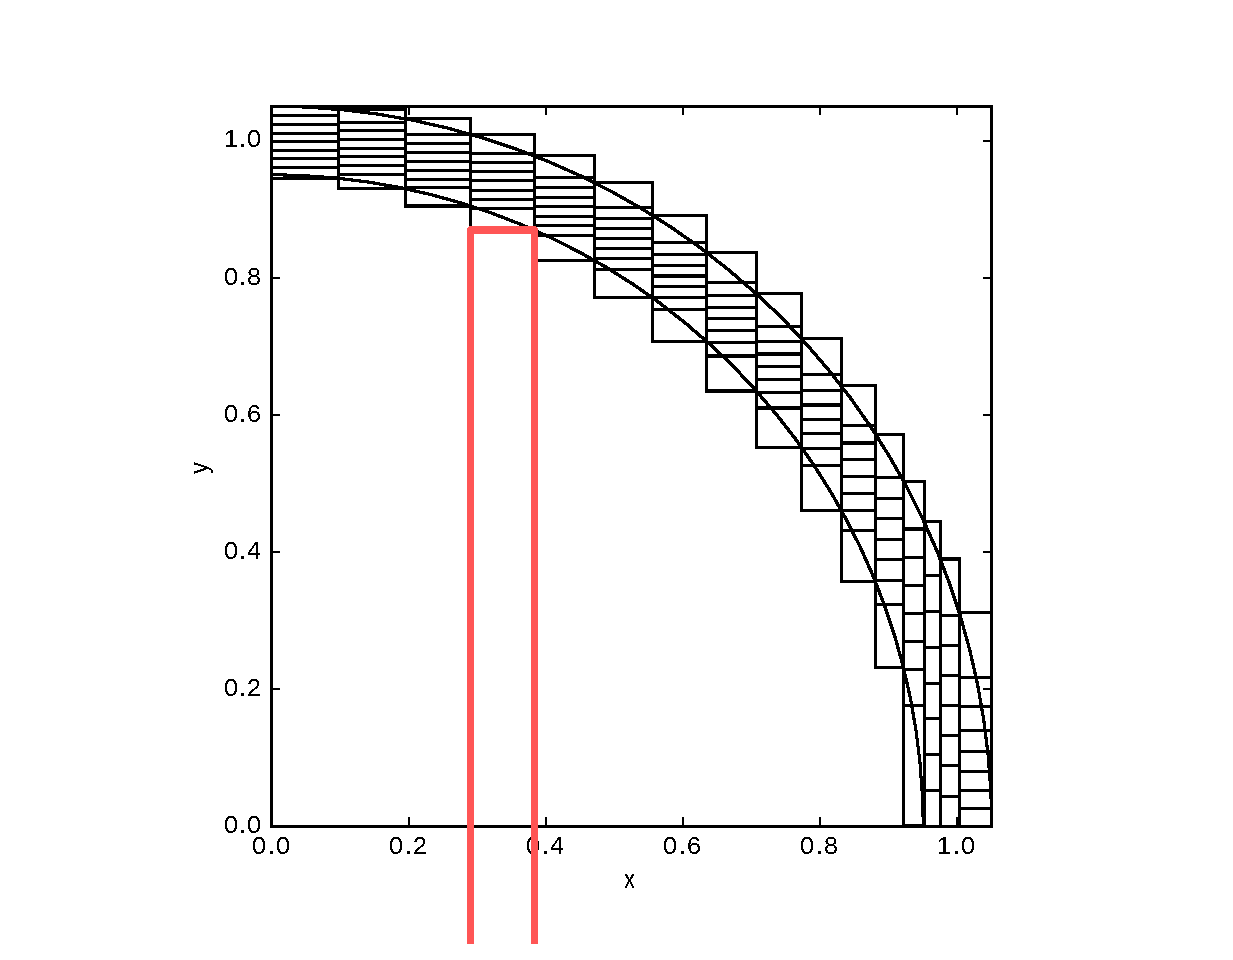
\includegraphics[width=8.6cm]{domain_cart.eps}
\end{center}
\end{minipage}
\begin{minipage}[b]{6cm}
\raggedright

細いリングを FDPS の標準の方法で領域分割するとすごく具合の悪いことが
起こる


\begin{itemize}

\item 細長い領域

\item 象限にまたがったものすごく大きな領域

\end{itemize}

通信が増えて計算効率が落ちる。

\end{minipage}

\pageheadl{解決方法}

\begin{minipage}[b]{9cm}
\begin{center}
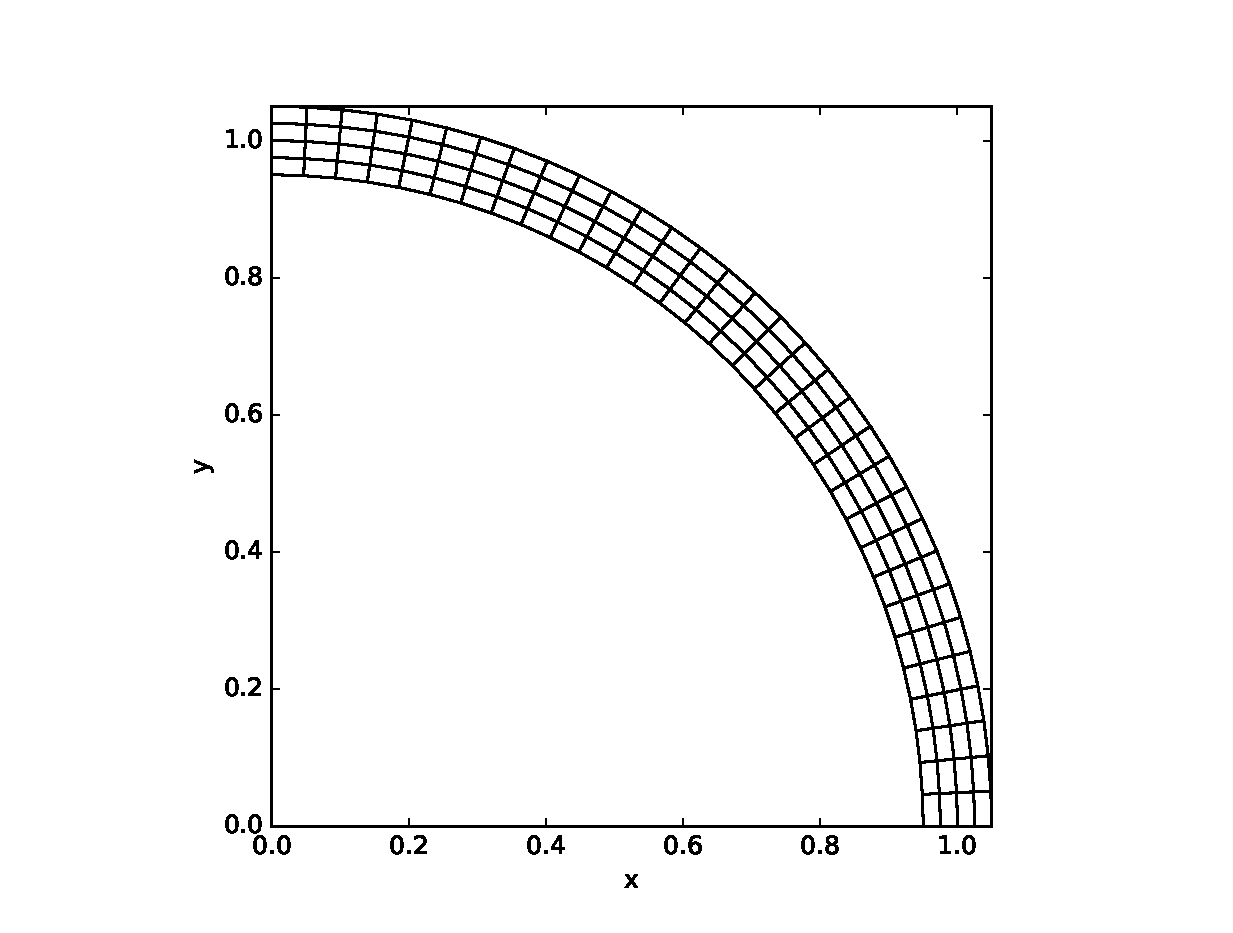
\includegraphics[width=8.6cm]{domain_cyl.eps}
\end{center}
\end{minipage}
\begin{minipage}[b]{6cm}
\raggedright

円柱座標なり極座標なりで領域分割すれば解決。
領域はほぼ長方形。正方形にもできる

\begin{itemize}

\item 通信が最小化

\item 座標系回転させてさらに粒子の移動を減らすことも

\end{itemize}


\end{minipage}


\pageheadl{実装の考え方}

\begin{itemize}

\item 領域分割、ツリー構築、ツリー辿る: 極座標または円筒座標で
\begin{itemize}
\item 非常に幅が広いリング: 半径方向を対数座標で
\item 局所的にはカーテシアンなので、粒子近傍でツリー辿ることはできる
\item 角度方向だけ周期境界
\end{itemize}
\item ツリーの物理量、相互作用計算はカーテシアンで
\item (現在のところ) 後者をユーザーコードで対応。
\begin{itemize}
\item FDPS の{\tt get\_pos} には極座標
\item 相互作用計算カーネルには別に物理量を
\item 4重極計算にはそれ用の FDPS の「モーメントクラス」追加する必要あ
り。sample/c++/planetary\_ring にサンプルあり。

\end{itemize}
\end{itemize}

\pageheadl{使い方}

割とややこしいので、sample/c++/planetary\_ring をみて下さい、、、

\pageheadl{効果}

\begin{itemize}

\item ノード数がすごく多い時には、「動くか動かないか」くらい違う: 象限
にまたがった領域とかがなくなるため

\item ノード数少ないとまああんまり、、、

\end{itemize}


\pageheadl{高度なシミュレーションコードの紹介}


\begin{itemize}

\item GPLUM: 惑星形成シミュレーション用 N体コード
https://github.com/YotaIshigaki/GPLUM
\begin{itemize}
\item $\rm P^3T$ スキーム使ってて速い。富岳でも(なんかとまる問題はある
が)動く。
\end{itemize}
\item PeTar: 球状星団シミュレーション用 N体コード
https://github.com/lwang-astro/PeTar
\begin{itemize}
\item $\rm P^3T$ スキーム使ってて速い。球状星団で連星の扱いもちゃんと
できて大規模並列化できてるのは世界でこれだけ
\end{itemize}
\item FDPS\_SPH: 巨大衝突とかできる自己重力SPHコード
https://github.com/NatsukiHosono/FDPS\_SPH

\item planetary\_ring: 大粒子数・大規模並列でちゃんと動くグローバルな惑星リングコード
FDPS 7.0 の sample/c++/planetary\_ring

\end{itemize}

それぞれ、世界トップクラスの計算ができるコードなので、目的にあってれば
これらの利用も御検討をみたいな。

DEM コードもそのうちに。



\end{document}

\begin{itemize}
\item 共通 
\begin{itemize}
\item 14:40-14:50  休憩・ZOOMつなぎ直し
\item 14:50-15:20 PIKGおよびFDPSの新機能について(牧野)
\item 15:20-16:55 6.実習・質問 (必要に応じてブレイクアウト利用)
\item 16:55-17:00  7. 結び(牧野)
\end{itemize}

\end{itemize}

\pagehead{イントロダクション残り:\\FDPS は何をするか?}


というよりむしろ、何がしたくない(やったことがない)人のためのものか:

\begin{itemize}

\item MPI でプログラム書いたことない

\item キャッシュ再利用のためのわけのわからないループ分割とかしたくない

\item 通信量減らすためにわけのわからない最適化とかするのも勘弁して欲し
い

\item SIMD 命令がでるようにコードをいじりまわすとか無理

\item 機械毎にどういう最適化すればいいか全然違うとか、それ以前に言語から違うとかはもういやだ

\end{itemize}

\pageheadl{そうはいっても---ではどうするか?}

昔からある考え方はこんな感じ?

\begin{itemize}

\item 並列化コンパイラになんとかしてもらう

\item 共有メモリハードウェアになんとかしてもらう

\item 並列言語とコンパイラの組み合わせになんとかしてもらう

\end{itemize}

しかし……
\begin{itemize}

\item 若い人はそういう考え方があったことも既に知らないような気がする。「スパ
コンとはそういうものだ」みたいな。

\item つまり、こういうアプローチはほぼ死滅した。

\item 理由は簡単: 性能がでない。安価なハードウェアで高い性能がでるものがプロ
グラミングが大変でも長期的には生き残る。

\end{itemize}

\pageheadl{じゃあ本当のところどうするか?}

\begin{enumerate}

\item 人生そういうものだと諦めて MPI でプログラム書いて最適化もする\\
難点: 普通の人の場合性能がでない。難しいことをしようとすると無限に時間
がかかって人生が終わってしまう。


\item 他人(学生、ポスドク、外注、ベンダ等)にMPI でプログラム書かせて最
適化もさせる\\
難点: 他人が普通の人の場合、やはり性能でない。無限に人と時間とお金がかかる。
あとでいじるにも無限に人と時間とお金がかかる。

\end{enumerate}

\begin{itemize}
\item どちらも今一つというか今百くらいである。

\item もちろん、「普通でない人」を確保できればなんとかなるがこれは希少
資源である。

\end{itemize}


\begin{shadebox}
原理的には、「普通でない人」を有効利用すればいい?
\end{shadebox}


%% \pagehead{どうやって有効利用するか?}

%% 色々な考え方がありえるが、我々の(というか私の)考え方:

%% \begin{itemize}

%% \item 「普通でない人」がやった方法を一般化して、色々な問題に適用する。
%% \item 例えば「粒子系一般」という程度
%% \item DRY (Don't Repeat Yourself) の原則の徹底


%% \end{itemize}


\pagehead{どうやって有効利用するか?}

色々な考え方がありえるが、我々の考え方:

\begin{itemize}

\item 「普通でない人」がやった方法を一般化して、色々な問題に適用する。
\item 例えば「粒子系一般」という程度
\item DRY (Don't Repeat Yourself) の原則の徹底
\item 理研CCS粒子系シミュレータ開発チームで詳細仕様策定及び実装

\end{itemize}

%% \newpage

%% \includegraphics[width=12cm]{../sph/teamphoto.eps}

%% \large

%% 細野\ \ \ 村主\ \ \ 岩澤\ \ \ 丸山\ \ \ 似鳥\\
%% 山本\ \ \ Barnes\ \ \ 牧野\ \ \ 谷川\ \ \ Rieder

%% +坪内(テクニカルスタッフ)、若松(アシスタント)

\pagehead{もうちょっと具体的には?}

色々な粒子系計算

\begin{itemize}

\item 重力多体系

\item 分子動力学

\item 粒子法による流体(SPH、MPS、MLS、その他)
\item 構造解析等のメッシュフリー法

\end{itemize}

計算のほとんどは近傍粒子との相互作用(遠距離力: Tree, FMM, PME その他)


\pagehead{もうちょっと具体的には?}

なので、粒子と相互作用の定義を与えると

\begin{itemize}

\item 領域分割(ロードバランスも考慮した)

\item 粒子の移動

\item ツリー法での相互作用の計算(そのために必要な通信も)

\item {\red 相互作用計算の SIMD化やGPGPU を利用するコード生成(Ver 6.0新機能)}
\item {\red 円盤系向けの効率よい並列化コード生成(Ver 7.0新機能)}

\end{itemize}

を高い効率(実行効率・並列化効率)でやってくれるプログラムを「自動生成」
できればいい。時間積分とかは自分で書く。

(独立時間刻み? $\rm P^3T$ スキームで)

ということで、詳しくはこれからの説明をどぞ。
\end{document}

\pagehead{実装方針}

\begin{itemize}

\item API は C++ で定義

\item ユーザーは

\begin{itemize}

\item 粒子データクラス

\item 粒子間相互作用を計算する関数(現在のところ、ユーザーが機種毎に最
適化。この自動生成は並行して開発中)

\end{itemize}

を用意。さらにドライバープログラム(I/Oライブラリコール等も含む)、時間
積分関数とかも書く 

\item 全体をコンパイルすると空間分割して粒子再配置して時間積分して、、、
というプログラムになる

\end{itemize}


\pagehead{開発の現状}

\begin{itemize}

\item 公開した (https://github.com/FDPS/FDPS/)

\item 同一のユーザープログラムで、シングルスレッドでもマルチスレッドで
もMPI並列でも動く。

\item 動くだけでなく、並列化効率は「非常に良い」

\item 重力多体(Barnes-Hut ツリー)、重力+SPH が「京」全ノードくらい(計
算時間が、、、)までで動作、重力(遠距離相互作用)は数万ノードでも実行効率高い。SPH(近
距離相互作用)は改良中


\item 多数のユーザーから喜びのお手紙を(ちょっと嘘)

\item GPU 対応、 Fortran 対応を公開

\end{itemize}

\href{file:///home2/home/makino/src/fdps/fdps/doc/doc_tutorial.pdf}{チュートリアル}


\pagehead{空間分割と並列化}

\begin{minipage}[b]{9cm}
\begin{center}
\includegraphics[width=8.6cm]{/home2/home/makino/papers/ishiyama/treepm/fig1.ps}
\end{center}
\end{minipage}
\begin{minipage}[b]{6.5cm}
空間分割して計算ノードに割り当て

Recursive Multisection (JM 2004)

\bigskip


「京」の Tofu ネットワークに適した方法

\bigskip


計算時間が均等になるよう領域サイズ調整(石山他 2009、2012)

\bigskip



\end{minipage}

領域サイズ調整アルゴリズムを数万ノードでもボトルネックにならないよう改
良(岩澤他 2015)

\pagehead{重力多体計算のサンプルユーザーコード(C++版)}

1. ヘッダと粒子クラス

\begin{verbatim}
#include <particle_simulator.hpp> //必須
using namespace PS;  //コードを簡潔に、、、、

class Nbody{            //名前は自由
public:
    F64    mass, eps;   //名前は自由
    F64vec pos, vel, acc; //名前は自由
    F64vec getPos() const {return pos;} //必須
    F64 getCharge() const {return mass;}//必須
    void copyFromFP(const Nbody &in){   //必須
        mass = in.mass;
        pos  = in.pos;
        eps  = in.eps;
    }
    void copyFromForce(const Nbody &out) { //必須
        acc = out.acc;
    }    
\end{verbatim}

\pagehead{粒子クラス(2)}

\begin{verbatim}
    void clear() { //必須
        acc = 0.0;
    }
    void readAscii(FILE *fp) {//FDPSのI/O使うなら
        fscanf(fp,
               "%lf%lf%lf%lf%lf%lf%lf%lf",
               &mass, &eps,
               &pos.x, &pos.y, &pos.z,
               &vel.x, &vel.y, &vel.z);
    }
    void predict(F64 dt) { //ユーザー利用
        vel += (0.5 * dt) * acc;
        pos += dt * vel;
    }
    void correct(F64 dt) { //ユーザー利用
        vel += (0.5 * dt) * acc;
    }
};
\end{verbatim}    


\pagehead{相互作用関数}
\begin{verbatim}
template <class TPJ>
struct CalcGrav{
    void operator () (const Nbody * ip,
                      const S32 ni,
                      const TPJ * jp,
                      const S32 nj,
                      Nbody * force) {
        for(S32 i=0; i<ni; i++){
            F64vec xi  = ip[i].pos;
            F64    ep2 = ip[i].eps
                * ip[i].eps;
            F64vec ai = 0.0;
\end{verbatim}    
\pagehead{相互作用関数(続き)}
\begin{verbatim}
            for(S32 j=0; j<nj;j++){
                F64vec xj = jp[j].pos;
                F64vec dr = xi - xj;
                F64 mj  = jp[j].mass;
                F64 dr2 = dr * dr + ep2;
                F64 dri = 1.0 / sqrt(dr2);                
                ai -= (dri * dri * dri
                       * mj) * dr;
            }
            force[i].acc += ai;
        }
    }
};
\end{verbatim}    
\pagehead{時間積分(ユーザープログラム内)}
\begin{verbatim}

template<class Tpsys>
void predict(Tpsys &p,
             const F64 dt) {
    S32 n = p.getNumberOfParticleLocal();
    for(S32 i = 0; i < n; i++)
        p[i].predict(dt);
}

template<class Tpsys>
void correct(Tpsys &p,
             const F64 dt) {
    S32 n = p.getNumberOfParticleLocal();
    for(S32 i = 0; i < n; i++)
        p[i].correct(dt);
}
\end{verbatim}



\pagehead{ユーザーの相互作用計算関数}
\begin{verbatim}
template <class TDI, class TPS, class TTFF>
void calcGravAllAndWriteBack(TDI &dinfo,
                             TPS &ptcl,
                             TTFF &tree) {
    dinfo.decomposeDomainAll(ptcl);
    ptcl.exchangeParticle(dinfo);    
    tree.calcForceAllAndWriteBack
        (CalcGrav<Nbody>(),
         CalcGrav<SPJMonopole>(),
         ptcl, dinfo);    
}
\end{verbatim}

ここで FDPS の関数群を使っている。
\pagehead{ユーザープログラム本体}
\begin{verbatim}
int main(int argc, char *argv[]) {
    F32 time  = 0.0;
    const F32 tend  = 10.0;
    const F32 dtime = 1.0 / 128.0;
    // FDPS 初期化
    PS::Initialize(argc, argv);
    PS::DomainInfo dinfo;
    dinfo.initialize();
    PS::ParticleSystem<Nbody> ptcl;
    ptcl.initialize();
    // FDPS に相互作用関数を渡す
    PS::TreeForForceLong<Nbody, Nbody,
        Nbody>::Monopole grav;
    grav.initialize(0);
    // 粒子データ読み込み
    ptcl.readParticleAscii(argv[1]);
\end{verbatim}    
\pagehead{ユーザープログラム本体}
\begin{verbatim}
    // 相互作用計算
    calcGravAllAndWriteBack(dinfo,
                            ptcl,
                            grav);
    while(time < tend) {
        predict(ptcl, dtime);        
        calcGravAllAndWriteBack(dinfo,
                                ptcl,
                                grav);
        correct(ptcl, dtime);        
        time += dtime;
    }
    PS::Finalize();
    return 0;
}
\end{verbatim}    

\pagehead{コメント等}

\begin{itemize}

\item 粒子クラスに謎関数があるのは、本来の粒子クラスと相互作用計算に最
    適化した粒子クラスを別に定義できるようにするため。
\item 粒子種も複数定義可能(ダークマターと流体等)。このために
相互作用を定義するところが若干複雑

\item ユーザー定義の相互作用計算は今のところアーキテクチャ向け最適化が
性能出すためには
必須。

\item 高度に最適化された並列化ツリーアルゴリズムを 150行くらいのユーザー
プログラムで使える。


\end{itemize}

\pagehead{まとめ}

\begin{itemize}

\item 粒子法は天体物理・惑星科学で色々使われている

\item が、問題点も結構沢山ある。
\begin{itemize}

\item 接触不連続で適合的でない
\item 並列化が結構困難
\end{itemize}

\item 前者は「改善」するスキームを開発したがまだ問題は残る

\item 後者は「汎用フレームワーク」で解決した(?)

\item 高粘性流体にも適用できる計算スキームを開発した。これからもうちょっと実験。


\end{itemize}


\end{document}

